The random subset problem randomly partitions network space into consensus sets, imposing a subset-sum constraint on consensus set sizes. In the context of symmetric load where all nodes request $|\mathcal{C}|$ consensus load the net consensus load is,
\begin{align}
	L = |\mathcal{C}| \cdot |\mathcal{N}|.
\end{align}
This requires performing $|\mathcal{C}|$ independent re-partitionings within each of which every node will be assigned exactly once. Under this allocation every node both contributes and requests $|\mathcal{C}|$ units of work.

The \emph{consensus assignment problem} generalises the random subset problem to accommodate arbitrary consensus set sizes and asymmetric load, allowing nodes to contribute and request arbitrary consensus workload, a prerequisite for enabling a free consensus market.

Representing consensus assignment via \emph{consensus assignment graphs} (Sec.~\ref{sec:assign_graphs}) reflecting the contributed and requested load by nodes and consensus sets, the algorithm uniformly samples from the space of satisfying assignments (Sec.~\ref{sec:uniform_consensus_samp}), achieved by defining consensus assignment via its algebraic group structure (Sec.~\ref{sec:assign_group}) and uniformly sampling the group action acting on an initial graph assignment (Sec.~\ref{sec:initial_graph_assignment}), where the pseudo-random algorithm is seeded (Sec.~\ref{sec:random_bitstreams}) by a secure random variable established by the network (Sec.~\ref{sec:secure_shared_randomness}) to ensure consistent evaluation in a distributed context. The distributed algorithm for the consensus assignment problem is shown in Alg.~\ref{alg:uniform_consensus_sampling}.

\begin{algorithm}[H]
	\begin{algorithmic}
		\Function{DistConsensusSampling}{$\mathcal{N}$, $U$, $V$, $d$} $\to E$
		\State $\mathcal{X}_\mathcal{N} \gets \textsc{SecureSharedRandomness}(\mathcal{N})$
		\State $E \gets \textsc{CanonicalGraph}(U,V,d)$
		\State $E \gets \textsc{ConsensusShuffle}(\mathcal{X}_\mathcal{N}, E)$
		\State \Return $E$
		\EndFunction
	\end{algorithmic}
	\caption{Distributed algorithm for the consensus assignment problem. A secure shared random variable (Sec.~\ref{sec:secure_shared_randomness}), $\mathcal{X}_\mathcal{N}$, collectively established by the network, $\mathcal{N}$, seeds pseudo-random sampling (Sec.~\ref{sec:uniform_consensus_samp}) over consensus assignments, $E$, satisfying the consensus assignment graph constraints, $(U,V,d)$ (Sec.~\ref{sec:assign_graphs}).} \label{alg:uniform_consensus_sampling}
\end{algorithm}

\subsection{Consensus assignment graphs} \label{sec:assign_graphs}

\begin{figure}[!htb]
	\centering
	\begin{tikzpicture}[genericStyle, every node/.style={circle, draw, minimum size=2em}]
    \def\UVsep{2.8}

    \foreach \i in {1,...,5} {
            \node[draw=none] (a\i) at (0,-\i) {};
        }
    \foreach \i in {1,...,5} {
            \node[draw=none] (b\i) at (\UVsep,-\i) {};
        }

    \node[nodeNetworkStyle, rectangle, rounded corners=5pt, fit=(a1) (a5), inner sep=4pt] (rectU) {};
    \node[nodeConsensusStyle, rectangle, rounded corners=5pt, fit=(b1) (b5), inner sep=4pt] (rectV) {};

    \node[draw=none, above=-0.2em of rectU] (labelU) {$U$};
    \node[draw=none, above=-0.2em of rectV] (labelV) {$V$};
    \node[draw=none] at ($(labelU)!0.5!(labelV)$) {$E$};

    \node[nodeGrayStyle] (a1) at (0,-1) {};
    \node[nodeGrayStyle] (a2) at (0,-2) {$u_i$};
    \node[nodeGrayStyle] (a3) at (0,-3) {};
    \node[draw=none] (a4) at (0,-4) {\LARGE $\vdots$};
    \node[nodeGrayStyle] (a5) at (0,-5) {};

    \node[nodeGrayStyle] (b1) at (\UVsep,-1) {};
    \node[nodeGrayStyle] (b2) at (\UVsep,-2) {};
    \node[nodeGrayStyle] (b3) at (\UVsep,-3) {$v_j$};
    \node[draw=none] (b4) at (\UVsep,-4) {\LARGE $\vdots$};
    \node[nodeGrayStyle] (b5) at (\UVsep,-5) {};

    \foreach \i in {1,...,5} {
            \foreach \j in {1,...,5} {
                    \draw[graphNonEdgeStyle] ($(rectU.east |- a\i) + (0.01,0)$) -- ($(rectV.west |- b\j) + (-0.01,0)$);
                }
        }

    \draw[->, black, line width=0.8, line cap=round] (rectU.east |- a2) -- node[draw=none, draw=none, text=black, above=-1em,midway] {$e=(u_i,v_j)$} (rectV.west |- b3);
\end{tikzpicture}
	%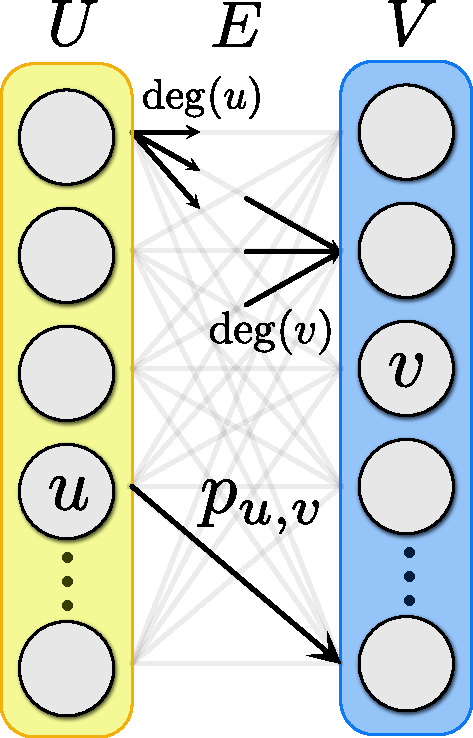
\includegraphics[width=0.4\columnwidth]{figs/bipartite_map.pdf}
	\caption{\textbf{Generalised consensus assignment problem.} Consensus assignment may be represented as a directed bipartite graph, \mbox{$\mathcal{G}=(U,V,E)$}, from a space of network nodes, $U\equiv\mathcal{N}$, to consensus sets, $V\equiv\{\mathcal{C}\}$, where vertex degree represents contributed/consumed consensus load. The set of all satisfying edge-sets $\{E\}$ represents the space of valid assignments. Under sampling, $p_{i,j}$ is the probability of the existence of edge \mbox{$e=(u_i,v_j)$}, which assigns node $u_i$ to consensus set $v_j$.}\label{fig:bipartite_map}
\end{figure}

\begin{figure}[!htb]
	\centering
	\resizebox{0.3\columnwidth}{!}{\begin{tikzpicture}[genericStyle, every node/.style={circle,draw,minimum size=2em}]
    \def\N{3}
    \def\nskip{8}
    \def\conn{2}
    \def\UVsep{2.5}

    \foreach \i in {1,...,\N} {
            \ifnum\i=\nskip
                \node[draw=none] (a\i) at (0,-\i) {\LARGE $\vdots$};
            \else
                \ifnum\i=\N
                    \node[nodeNetworkStyle] (a\i) at (0,-\i) {}; % $u_m$
                \else
                    \node[nodeNetworkStyle] (a\i) at (0,-\i) {}; % $u_{\i}$
                \fi
            \fi
        }
    \foreach \i in {1,...,\N} {
            \ifnum\i=\nskip
                \node[draw=none] (b\i) at (\UVsep,-\i) {\LARGE $\vdots$};
            \else
                \ifnum\i=\N
                    \node[nodeConsensusStyle] (b\i) at (\UVsep,-\i) {}; % $v_n$
                \else
                    \node[nodeConsensusStyle] (b\i) at (\UVsep,-\i) {}; % $v_{\i}$
                \fi
            \fi
        }

    \foreach \i in {1,...,\N} {
            \foreach \j in {1,...,\N} {
                    \ifnum\i=\nskip
                    \else
                        \ifnum\j=\nskip
                        \else
                            \draw[graphNonEdgeStyle] ($(a\i.east)$) -- ($(b\j.west)$);
                        \fi
                    \fi
                }
        }

    \draw[graphEdgeStyle] ($(a1.east)$) -- ($(b1.west)$);
    \draw[graphEdgeStyle] ($(a1.east)$) -- ($(b2.west)$);

    \draw[graphEdgeStyle] ($(a2.east)$) -- ($(b2.west)$);
    \draw[graphEdgeStyle] ($(a2.east)$) -- ($(b3.west)$);

    \draw[graphEdgeStyle] ($(a3.east)$) -- ($(b3.west)$);
    \draw[graphEdgeStyle] ($(a3.east)$) -- ($(b1.west)$);
\end{tikzpicture}}
	\hfill
	\resizebox{0.3\columnwidth}{!}{\begin{tikzpicture}[genericStyle, every node/.style={circle,draw,minimum size=2em}]
    \def\N{3}
    \def\nskip{8}
    \def\conn{2}
    \def\UVsep{2.5}
    
    \foreach \i in {1,...,\N} {
        \ifnum\i=\nskip
          \node[draw=none] (a\i) at (0,-\i) {\LARGE $\vdots$};
        \else
            \ifnum\i=\N
                \node[nodeUStyle] (a\i) at (0,-\i) {}; % $u_m$
            \else
                \node[nodeUStyle] (a\i) at (0,-\i) {}; % $u_{\i}$
            \fi
        \fi
    }
    \foreach \i in {1,...,\N} {
        \ifnum\i=\nskip
            \node[draw=none] (b\i) at (\UVsep,-\i) {\LARGE $\vdots$};
        \else
            \ifnum\i=\N
                \node[nodeVStyle] (b\i) at (\UVsep,-\i) {}; % $v_n$
            \else
                \node[nodeVStyle] (b\i) at (\UVsep,-\i) {}; % $v_{\i}$
            \fi
        \fi
    }
    
     \foreach \i in {1,...,\N} {
     	\foreach \j in {1,...,\N} {
               \ifnum\i=\nskip
                \else
                	\ifnum\j=\nskip
                    \else
                        \draw[graphNonEdgeStyle] ($(a\i.east)$) -- ($(b\j.west)$);
                    \fi
                \fi
        }
    }
    
    \draw[graphEdgeStyle] ($(a1.east)$) -- ($(b1.west)$);
    \draw[graphEdgeStyle] ($(a1.east)$) -- ($(b3.west)$);

    \draw[graphEdgeStyle] ($(a2.east)$) -- ($(b1.west)$);
    \draw[graphEdgeStyle] ($(a2.east)$) -- ($(b2.west)$);

    \draw[graphEdgeStyle] ($(a3.east)$) -- ($(b3.west)$);
    \draw[graphEdgeStyle] ($(a3.east)$) -- ($(b2.west)$);
\end{tikzpicture}}
	\hfill
	\resizebox{0.3\columnwidth}{!}{\begin{tikzpicture}[genericStyle, every node/.style={circle,draw,minimum size=2em}]
    \def\N{3}
    \def\nskip{8}
    \def\conn{2}
    \def\UVsep{2.5}

    \foreach \i in {1,...,\N} {
            \ifnum\i=\nskip
                \node[draw=none] (a\i) at (0,-\i) {\LARGE $\vdots$};
            \else
                \ifnum\i=\N
                    \node[nodeNetworkStyle] (a\i) at (0,-\i) {}; % $u_m$
                \else
                    \node[nodeNetworkStyle] (a\i) at (0,-\i) {}; % $u_{\i}$
                \fi
            \fi
        }
    \foreach \i in {1,...,\N} {
            \ifnum\i=\nskip
                \node[draw=none] (b\i) at (\UVsep,-\i) {\LARGE $\vdots$};
            \else
                \ifnum\i=\N
                    \node[nodeConsensusStyle] (b\i) at (\UVsep,-\i) {}; % $v_n$
                \else
                    \node[nodeConsensusStyle] (b\i) at (\UVsep,-\i) {}; % $v_{\i}$
                \fi
            \fi
        }

    \foreach \i in {1,...,\N} {
            \foreach \j in {1,...,\N} {
                    \ifnum\i=\nskip
                    \else
                        \ifnum\j=\nskip
                        \else
                            \draw[graphNonEdgeStyle] ($(a\i.east)$) -- ($(b\j.west)$);
                        \fi
                    \fi
                }
        }

    \draw[graphEdgeStyle] ($(a1.east)$) -- ($(b2.west)$);
    \draw[graphEdgeStyle] ($(a1.east)$) -- ($(b3.west)$);

    \draw[graphEdgeStyle] ($(a2.east)$) -- ($(b1.west)$);
    \draw[graphEdgeStyle] ($(a2.east)$) -- ($(b2.west)$);

    \draw[graphEdgeStyle] ($(a3.east)$) -- ($(b3.west)$);
    \draw[graphEdgeStyle] ($(a3.east)$) -- ($(b1.west)$);
\end{tikzpicture}}

	\vspace{10pt}

	\resizebox{0.3\columnwidth}{!}{\begin{tikzpicture}[genericStyle, every node/.style={circle,draw,minimum size=2em}]
    \def\N{3}
    \def\nskip{8}
    \def\conn{2}
    \def\UVsep{2.5}

    \foreach \i in {1,...,\N} {
            \ifnum\i=\nskip
                \node[draw=none] (a\i) at (0,-\i) {\LARGE $\vdots$};
            \else
                \ifnum\i=\N
                    \node[nodeNetworkStyle] (a\i) at (0,-\i) {}; % $u_m$
                \else
                    \node[nodeNetworkStyle] (a\i) at (0,-\i) {}; % $u_{\i}$
                \fi
            \fi
        }
    \foreach \i in {1,...,\N} {
            \ifnum\i=\nskip
                \node[draw=none] (b\i) at (\UVsep,-\i) {\LARGE $\vdots$};
            \else
                \ifnum\i=\N
                    \node[nodeConsensusStyle] (b\i) at (\UVsep,-\i) {}; % $v_n$
                \else
                    \node[nodeConsensusStyle] (b\i) at (\UVsep,-\i) {}; % $v_{\i}$
                \fi
            \fi
        }

    \foreach \i in {1,...,\N} {
            \foreach \j in {1,...,\N} {
                    \ifnum\i=\nskip
                    \else
                        \ifnum\j=\nskip
                        \else
                            \draw[graphNonEdgeStyle] ($(a\i.east)$) -- ($(b\j.west)$);
                        \fi
                    \fi
                }
        }

    \draw[graphEdgeStyle] ($(a1.east)$) -- ($(b1.west)$);
    \draw[graphEdgeStyle] ($(a1.east)$) -- ($(b2.west)$);

    \draw[graphEdgeStyle] ($(a2.east)$) -- ($(b1.west)$);
    \draw[graphEdgeStyle] ($(a2.east)$) -- ($(b3.west)$);

    \draw[graphEdgeStyle] ($(a3.east)$) -- ($(b2.west)$);
    \draw[graphEdgeStyle] ($(a3.east)$) -- ($(b3.west)$);
\end{tikzpicture}}
	\hfill
	\resizebox{0.3\columnwidth}{!}{\begin{tikzpicture}[genericStyle, every node/.style={circle,draw,minimum size=2em}]
    \def\N{3}
    \def\nskip{8}
    \def\conn{2}
    \def\UVsep{2.5}

    \foreach \i in {1,...,\N} {
            \ifnum\i=\nskip
                \node[draw=none] (a\i) at (0,-\i) {\LARGE $\vdots$};
            \else
                \ifnum\i=\N
                    \node[nodeNetworkStyle] (a\i) at (0,-\i) {}; % $u_m$
                \else
                    \node[nodeNetworkStyle] (a\i) at (0,-\i) {}; % $u_{\i}$
                \fi
            \fi
        }
    \foreach \i in {1,...,\N} {
            \ifnum\i=\nskip
                \node[draw=none] (b\i) at (\UVsep,-\i) {\LARGE $\vdots$};
            \else
                \ifnum\i=\N
                    \node[nodeConsensusStyle] (b\i) at (\UVsep,-\i) {}; % $v_n$
                \else
                    \node[nodeConsensusStyle] (b\i) at (\UVsep,-\i) {}; % $v_{\i}$
                \fi
            \fi
        }

    \foreach \i in {1,...,\N} {
            \foreach \j in {1,...,\N} {
                    \ifnum\i=\nskip
                    \else
                        \ifnum\j=\nskip
                        \else
                            \draw[graphNonEdgeStyle] ($(a\i.east)$) -- ($(b\j.west)$);
                        \fi
                    \fi
                }
        }

    \draw[graphEdgeStyle] ($(a1.east)$) -- ($(b1.west)$);
    \draw[graphEdgeStyle] ($(a1.east)$) -- ($(b3.west)$);

    \draw[graphEdgeStyle] ($(a2.east)$) -- ($(b2.west)$);
    \draw[graphEdgeStyle] ($(a2.east)$) -- ($(b3.west)$);

    \draw[graphEdgeStyle] ($(a3.east)$) -- ($(b1.west)$);
    \draw[graphEdgeStyle] ($(a3.east)$) -- ($(b2.west)$);
\end{tikzpicture}}
	\hfill
	\resizebox{0.3\columnwidth}{!}{\begin{tikzpicture}[genericStyle, every node/.style={circle,draw,minimum size=2em}]
    \def\N{3}
    \def\nskip{8}
    \def\conn{2}
    \def\UVsep{2.5}

    \foreach \i in {1,...,\N} {
            \ifnum\i=\nskip
                \node[draw=none] (a\i) at (0,-\i) {\LARGE $\vdots$};
            \else
                \ifnum\i=\N
                    \node[nodeNetworkStyle] (a\i) at (0,-\i) {}; % $u_m$
                \else
                    \node[nodeNetworkStyle] (a\i) at (0,-\i) {}; % $u_{\i}$
                \fi
            \fi
        }
    \foreach \i in {1,...,\N} {
            \ifnum\i=\nskip
                \node[draw=none] (b\i) at (\UVsep,-\i) {\LARGE $\vdots$};
            \else
                \ifnum\i=\N
                    \node[nodeConsensusStyle] (b\i) at (\UVsep,-\i) {}; % $v_n$
                \else
                    \node[nodeConsensusStyle] (b\i) at (\UVsep,-\i) {}; % $v_{\i}$
                \fi
            \fi
        }

    \foreach \i in {1,...,\N} {
            \foreach \j in {1,...,\N} {
                    \ifnum\i=\nskip
                    \else
                        \ifnum\j=\nskip
                        \else
                            \draw[graphNonEdgeStyle] ($(a\i.east)$) -- ($(b\j.west)$);
                        \fi
                    \fi
                }
        }

    \draw[graphEdgeStyle] ($(a1.east)$) -- ($(b2.west)$);
    \draw[graphEdgeStyle] ($(a1.east)$) -- ($(b3.west)$);

    \draw[graphEdgeStyle] ($(a2.east)$) -- ($(b1.west)$);
    \draw[graphEdgeStyle] ($(a2.east)$) -- ($(b3.west)$);

    \draw[graphEdgeStyle] ($(a3.east)$) -- ($(b1.west)$);
    \draw[graphEdgeStyle] ($(a3.east)$) -- ($(b2.west)$);
\end{tikzpicture}}
	\caption{\textbf{Satisfying solutions for the consensus assignment problem.} The space of satisfying graphs assignments, \mbox{$\{\mathcal{G}\} = C_d\times \mathcal{G}_{n,d}$}, for $n=3$ nodes of degree $d=2$.} \label{fig:edge_assignments}
\end{figure}

Consider a directed bipartite graph (Fig.~\ref{fig:bipartite_map}),
\begin{align}
	\mathcal{G} = (U,V,E),
\end{align}
where vertices $u\in U$ and $v\in V$ represent network nodes (\mbox{$U=\mathcal{N}$}) and consensus sets (\mbox{$V=\mathcal{\{\mathcal{C}\}}$}) respectively, and the directed edge set $E$ defines the assignment of nodes to consensus sets where each edge is associated with a unit of consensus work. The constraint that nodes may be assigned at most once to a given consensus set imposes that $G$ is a simple graph.

Consensus load may be arbitrarily partitioned and nodes may make multiple requests for consensus sets, hence in general $|\mathcal{S}|\neq|\{\mathcal{C}\}|$. %Expressing vertex sets as degree sequences,
%\begin{align}
%	U &= (\mathrm{deg}(u_1),\dots,\mathrm{deg}(u_{|U|})), \nonumber\\
%	V &= (\mathrm{deg}(v_1),\dots,\mathrm{deg}v_{|V|})),
%\end{align}

Vertex degrees represent workload, where $\mathrm{deg}(u)$ denotes work contributed by node $u$ and $\mathrm{deg}(v)$ the load requested by consensus set $v$. The degree sum formula for bipartite graphs equates to a conservation of work constraint in the system,
\begin{align} \label{eq:degree_sum}
	\sum_{u\in U} \mathrm{deg}(u) = \sum_{v\in V} \mathrm{deg}(v) = |E|,
\end{align}
where $|E|$ represents net consensus work.

Asymmetric load introduces sampling bias into the average-case likelihood of compromise, $r$, defined in Eq.~\eqref{eq:av_r_uniform}, which generalises to,
\begin{align}
	r = \frac{1}{|E|} \sum_{i=1}^{|\mathcal{N}|} \mathrm{deg}(u_i) \cdot r_i.
\end{align}

The assignment of network nodes to consensus sets is equivalent to assigning edge-sets $E$ subject to the constraints imposed by the degree sequence,
\begin{align} \label{eq:degree_seq}
	d = ( & \mathrm{deg}(u_1),\dots,\mathrm{deg}(u_{|U|});\nonumber \\
	      & \mathrm{deg}(v_1),\dots,\mathrm{deg}(v_{|V|})),
\end{align}
where,
\begin{align}
	|d| = |U|+|V| = |\mathcal{N}|+|\{\mathcal{C}\}|.
\end{align}
Expressing graphs by their edge-sets, $E$,
\begin{align}
	\mathcal{G} = \{(u_e\in U, v_e\in V)\}_{e\in E},
\end{align}
where edges $(u_e,v_e)$ denote the assignment of node $u_e$ to consensus set $v_e$. In columnar representation,
\begin{align}
	E_U & = \{u_e\}_{e\in E},\nonumber \\
	E_V & = \{v_e\}_{e\in E},
\end{align}
elements have multiplicity given by their degree.

\subsubsection{Initial assignment} \label{sec:initial_graph_assignment}

\begin{figure}[!htb]
	\centering
	\resizebox{0.75\columnwidth}{!}{
		\begin{tikzpicture}[genericStyle]
    \def\N{10}
    \def\nskip{7}
    \def\conn{5}
    \def\UVsep{5}
    
    \foreach \i in {1,...,\N} {
        \ifnum\i=\nskip
          \node[draw=none] (a\i) at (0,-\i) {\LARGE $\vdots$};
        \else
            \ifnum\i=\N
                \node[nodeUStyle] (a\i) at (0,-\i) {}; % $u_m$
            \else
                \node[nodeUStyle] (a\i) at (0,-\i) {}; % $u_{\i}$
            \fi
        \fi
    }
    \foreach \i in {1,...,\N} {
        \ifnum\i=\nskip
            \node[draw=none] (b\i) at (\UVsep,-\i) {\LARGE $\vdots$};
        \else
            \ifnum\i=\N
                \node[nodeVStyle] (b\i) at (\UVsep,-\i) {}; % $v_n$
            \else
                \node[nodeVStyle] (b\i) at (\UVsep,-\i) {}; % $v_{\i}$
            \fi
        \fi
    }
    
     \foreach \i in {1,...,\N} {
     	\foreach \j in {1,...,\N} {
               \ifnum\i=\nskip
                \else
                	\ifnum\j=\nskip
                    \else
                        \draw[graphNonEdgeStyle] ($(a\i.east)$) -- ($(b\j.west)$);
                    \fi
                \fi
        }
    }

    
    \foreach \i in {1,...,\N} {
        \foreach \offset in {1,...,\conn} {
            \pgfmathtruncatemacro{\target}{mod(\i+\offset-2,\N)+1}
                \ifnum\i=\nskip
                \else
                \ifnum\target=\nskip
                    \else
                        \draw[graphEdgeStyle] ($(a\i.east)$) -- ($(b\target.west)$);
                    \fi
                \fi
        }
    }
    
  	\foreach \j in {1,...,\conn} {
                        \draw[-,redHighlightColor,line width=2,line cap=round] ($(a1.east)$) -- ($(b\j.west)$);
        }

    \node[draw=none] at ($(a1)!0.5!(b1) + (0,0.3)$) {$\mathcal{G}_{n,d}$};

    \coordinate (bracetop) at ($(b1.east) + (1em,0)$);
    \coordinate (bracetopin) at ($(bracetop) + (-0.1,0)$);
    \coordinate (bracebott) at ($(b\conn.east) + (1em,0)$);
    \coordinate (bracebottin) at ($(bracebott) + (-0.1,0)$);
    \draw[redHighlightColor, line width=1.5] (bracetopin) -- (bracetop) -- (bracebott) -- (bracebottin);

        \node[draw=none] at ($(bracetop)!0.5!(bracebott) + (3.5em,0)$) {$d=N(r/p,\varepsilon)$};
\end{tikzpicture}
	}
	\caption{\textbf{Uniform bidding initial assignment graph.} \mbox{$\mathcal{G}_{n,d}$ has $n$ nodes and $n$ consensus sets, all with degree $d$.}}\label{fig:butterfly_graph}
\end{figure}

\begin{figure}[!htb]
	\centering
	\resizebox{0.31\columnwidth}{!}{
    \begin{tikzpicture}[genericStyle]
        \def\N{6}
        \def\nskip{8}
        \def\conn{1}
        \def\UVsep{2.8}

        \foreach \i in {1,...,\N} {
                \ifnum\i=\nskip
                    \node[draw=none] (a\i) at (0,-\i) {\LARGE $\vdots$};
                \else
                    \ifnum\i=\N
                        \node[nodeNetworkStyle] (a\i) at (0,-\i) {}; % $u_m$
                    \else
                        \node[nodeNetworkStyle] (a\i) at (0,-\i) {}; % $u_{\i}$
                    \fi
                \fi
            }
        \foreach \i in {1,...,\N} {
                \ifnum\i=\nskip
                    \node[draw=none] (b\i) at (\UVsep,-\i) {\LARGE $\vdots$};
                \else
                    \ifnum\i=\N
                        \node[nodeConsensusStyle] (b\i) at (\UVsep,-\i) {}; % $v_n$
                    \else
                        \node[nodeConsensusStyle] (b\i) at (\UVsep,-\i) {}; % $v_{\i}$
                    \fi
                \fi
            }


        \foreach \i in {1,...,\N} {
                \foreach \j in {1,...,\N} {
                        \ifnum\i=\nskip
                        \else
                            \ifnum\j=\nskip
                            \else
                                \draw[graphNonEdgeStyle] ($(a\i.east)$) -- ($(b\j.west)$);
                            \fi
                        \fi
                    }
            }

        \foreach \i in {1,...,\N} {
                \foreach \offset in {1,...,\conn} {
                        \pgfmathtruncatemacro{\target}{mod(\i+\offset-2,\N)+1}
                        \ifnum\i=\nskip
                        \else
                            \ifnum\target=\nskip
                            \else
                                \draw[graphEdgeStyle] ($(a\i.east)$) -- ($(b\target.west)$);
                            \fi
                        \fi
                    }
            }

        \node[draw=none] at ($(a1)!0.5!(b1) + (0,0.5)$) {\large $\mathcal{G}_{6,1}$};
    \end{tikzpicture}
}
	\hfill
	\resizebox{0.31\columnwidth}{!}{
\begin{tikzpicture}[genericStyle]
    \def\N{6}
    \def\nskip{8}
    \def\conn{3}
    \def\UVsep{2.8}
    
    \foreach \i in {1,...,\N} {
        \ifnum\i=\nskip
          \node[draw=none] (a\i) at (0,-\i) {\LARGE $\vdots$};
        \else
            \ifnum\i=\N
                \node[nodeUStyle] (a\i) at (0,-\i) {}; % $u_m$
            \else
                \node[nodeUStyle] (a\i) at (0,-\i) {}; % $u_{\i}$
            \fi
        \fi
    }
    \foreach \i in {1,...,\N} {
        \ifnum\i=\nskip
            \node[draw=none] (b\i) at (\UVsep,-\i) {\LARGE $\vdots$};
        \else
            \ifnum\i=\N
                \node[nodeVStyle] (b\i) at (\UVsep,-\i) {}; % $v_n$
            \else
                \node[nodeVStyle] (b\i) at (\UVsep,-\i) {}; % $v_{\i}$
            \fi
        \fi
    }
    
    
     \foreach \i in {1,...,\N} {
     	\foreach \j in {1,...,\N} {
               \ifnum\i=\nskip
                \else
                	\ifnum\j=\nskip
                    \else
                        \draw[graphNonEdgeStyle] ($(a\i.east)$) -- ($(b\j.west)$);
                    \fi
                \fi
        }
    }
    
    \foreach \i in {1,...,\N} {
        \foreach \offset in {1,...,\conn} {
            \pgfmathtruncatemacro{\target}{mod(\i+\offset-2,\N)+1}
                \ifnum\i=\nskip
                \else
                \ifnum\target=\nskip
                    \else
                        \draw[graphEdgeStyle] ($(a\i.east)$) -- ($(b\target.west)$);
                    \fi
                \fi
        }
    }

    \node[draw=none] at ($(a1)!0.5!(b1) + (0,0.5)$) {\large $\mathcal{G}_{6,3}$};
\end{tikzpicture}
}
	\hfill
	\resizebox{0.31\columnwidth}{!}{
\begin{tikzpicture}[genericStyle]
    \def\N{6}
    \def\nskip{8}
    \def\conn{6}
    \def\UVsep{2.8}
    
    \foreach \i in {1,...,\N} {
        \ifnum\i=\nskip
          \node[draw=none] (a\i) at (0,-\i) {\LARGE $\vdots$};
        \else
            \ifnum\i=\N
                \node[nodeUStyle] (a\i) at (0,-\i) {}; % $u_m$
            \else
                \node[nodeUStyle] (a\i) at (0,-\i) {}; % $u_{\i}$
            \fi
        \fi
    }
    \foreach \i in {1,...,\N} {
        \ifnum\i=\nskip
            \node[draw=none] (b\i) at (\UVsep,-\i) {\LARGE $\vdots$};
        \else
            \ifnum\i=\N
                \node[nodeVStyle] (b\i) at (\UVsep,-\i) {}; % $v_n$
            \else
                \node[nodeVStyle] (b\i) at (\UVsep,-\i) {}; % $v_{\i}$
            \fi
        \fi
    }
    
    
     \foreach \i in {1,...,\N} {
     	\foreach \j in {1,...,\N} {
               \ifnum\i=\nskip
                \else
                	\ifnum\j=\nskip
                    \else
                        \draw[graphNonEdgeStyle] ($(a\i.east)$) -- ($(b\j.west)$);
                    \fi
                \fi
        }
    }
    
    \foreach \i in {1,...,\N} {
        \foreach \offset in {1,...,\conn} {
            \pgfmathtruncatemacro{\target}{mod(\i+\offset-2,\N)+1}
                \ifnum\i=\nskip
                \else
                \ifnum\target=\nskip
                    \else
                        \draw[graphEdgeStyle] ($(a\i.east)$) -- ($(b\target.west)$);
                    \fi
                \fi
        }
    }

    \node[draw=none] at ($(a1)!0.5!(b1) + (0,0.5)$) {\large $\mathcal{G}_{6,6}=K_{6,6}$};
\end{tikzpicture}
}
	\caption{\textbf{Uniform bidding initial assignment graph.} \mbox{$\mathcal{G}_{n,d}$} has $n$ nodes and $n$ consensus sets, all with degree $d$, where \mbox{$d\leq n$}. For \mbox{$n=d$} we obtain the complete bipartite graph \mbox{$\mathcal{G}_{n,n}=K_{n,n}$.}}\label{fig:butterfly_graph_comp}
\end{figure}

Uniformly sampling consensus allocation requires applying sampled consensus group transformations (Alg.~\ref{alg:consensus_shuffle}) to an initial satisfying graph assignment (Fig.~\ref{fig:bipartite_map}) --- a solution to the \emph{bipartite realisation problem}. Via the Gale-Ryser theorem \cite{Gale1957, Ryser1957}, realisable bipartite graphs (those with \emph{bigraphic} degree sequences) demands,
\begin{align} \label{eq:bipartite_real}
	\sum_{i=1}^{|U|} \mathrm{deg}(u_i) & = \sum_{j=1}^{|V|} \mathrm{deg}(v_j),                                                     \\
	\sum_{i=1}^k \mathrm{deg}(u_i)     & \leq \sum_{j=1}^{|V|} \min(\mathrm{deg}(v_j),k),\,\forall\, k\in\{1,\dots,|V|\},\nonumber
\end{align}
where the second constraint assumes $U$ and $V$ are ordered decreasingly by degree. Realisable bipartite graphs may be efficiently realised using the Havel-Hakimi algorithm \cite{Havel1955, Hakimi62}, shown in Alg.~\ref{alg:initial_assignment}, which we employ for initial canonical graph assignment.

%\footnote{In retrospect, the probability constraints imposed by Eq.~\eqref{eq:prob_cons} imply Alg.~\ref{alg:initial_assignment} directly affords a less sophisticated uniform sampling algorithm by replacing the inner for-loop with uniform selection of $\mathrm{deg}(u)$ vertices $v$ where \mbox{$\mathrm{deg}(v)>0$},\begin{align}\vec{v}'\gets\textsc{ChooseRandom}(\{\vec{v}_j\,|\, \mathrm{deg}(\vec{v}_j)>0\}_j,\mathrm{deg}(u)).\end{align}The author has a preference for the approach presented in the main text.}.

The simplest bidding format for ensuring realisable consensus assignment is \emph{uniform bidding} where all nodes request a single consensus set of size $|\mathcal{C}|$, and all vertices have constant degree,
\begin{align}
	\mathrm{deg}(u) = \mathrm{deg}(v)= |\mathcal{C}|,\,\,\forall\, u\in U, v\in V,
\end{align}
which is realisable as per Eq.~\eqref{eq:bipartite_real} if and only if,
\begin{align}
	|\mathcal{C}| \leq |\mathcal{N}'|,
\end{align}
where,
\begin{align}
	|U|=|V|=|\mathcal{N}'|=|\mathcal{C}|,
\end{align}
is the number of participating network nodes, equivalently the number of consensus sets. The same condition holds if all nodes request a constant number of consensus sets of uniform size.

\subsection{Uniform consensus sampling} \label{sec:uniform_consensus_samp}

Secure consensus assignment requires assigning edge-sets uniformly at random over the space of all satisfying edge-sets. Uniformity implies maximisation of entropy, given by,
\begin{align}
	H(C(d)) = \log_2(|C(d)|),
\end{align}
where $|C(d)|$ is the order of the respective consensus group. Degeneracies in permutations result in sampling bias thereby reducing entropy, requiring that algorithmic implementation does not double-count degenerate permutations from the symmetric group.

\subsubsection{Fisher-Yates shuffle}

The Fisher-Yates shuffle \cite{FisherYates53} is an efficient algorithm for applying in-place permutations $\pi\in S_n$ to an array of $n$ elements uniformly at random (Alg.~\ref{alg:fisher_yates}).

The algorithm iteratively allows every array index to randomly exchange itself with any element not already assigned. Assuming $O(1)$ random number generation the Fisher-Yates shuffle exhibits $O(n)$ time-complexity. As the operational primitive is the exchange operation the algorithm permutes arrays in-place.

The sequence of $O(n)$ random numbers chosen during execution defines a decision tree whose $i$th level assigns the $i$th array index. Individual execution paths correspond to individual permutations with a one-to-one correspondence. Hence, the algorithm's execution space $\mathcal{L}_n$ is isomorphic to the symmetric group,
\begin{align}
	\mathcal{L}_n \cong S_n,
\end{align}
under mapping between execution paths \mbox{$l\in\mathcal{L}_n$} and permutations \mbox{$\pi\in S_n$}. As all execution paths occur with uniform probability $1/n!$ the algorithm uniformly samples from the symmetric group.

\begin{algorithm}[H]
	\begin{algorithmic}
		\Function{FisherYatesShuffle}{$\vec{v}$} $\to \vec{v}$ \Comment{$O(n)$}
		\For{$i \gets |\vec{v}|-1 \textbf{ to } 1$} \Comment{$O(n)$}
		\State $j \gets \textsc{Random}(\{0,\dots,i\})$ \Comment{$O(1)$}
		\State $v_i\leftrightarrow v_j$ \Comment{Exchange}
		\EndFor
		\State \Return $\vec{v}$
		\EndFunction
	\end{algorithmic}
	\caption{\cite{FisherYates53} The Fisher-Yates shuffle algorithm for applying a random permutation $\pi\in S_{|\vec{v}|}$ to the elements a vector $\vec{v}$. The algorithm permutes  vectors in-place with $O(n)$ runtime assuming an $O(1)$ \textsc{Random}($\cdot$) function.}\label{alg:fisher_yates}
\end{algorithm}

The uniqueness of execution paths may be seen by noting that an element at index $j\leq i$ has  exactly one path to be reassigned to index $i$, via the direct exchange $v_i\leftrightarrow v_j$ when the loop reaches index $i$.

The execution path $l\in\mathcal{L}_n$ of the algorithm directly relates to the cycle decomposition of the respective group element. As the algorithm iterates through $i$ the series of exchange operations defines a path. When a trivial $v_i\leftrightarrow v_i$ exchange occurs it terminates that path, closing it as a cycle, after which the next $i$ opens a new one.

Closely related to the Fisher-Yates shuffle is Sattolo's algorithm \cite{Sattolo86} for uniformly sampling the cyclic group ($C_n$) differing only from the Fisher-Yates shuffle in the set of allowed exchanges,
\begin{align}
	\text{Fisher-Yates }(S_n):\,\, & 0\leq j\leq i,\nonumber \\
	\text{Sattolo }(C_n):\,\,      & 0\leq j<i.
\end{align}
Note that this distinction serves to prohibit trivial exchanges ($v_i\leftrightarrow v_i$) thereby forcing all execution paths to define single cycles.

\subsubsection{Graph randomisation}

* Graph is $N_C$-regular.

* Probability of node $u\in U$ being assigned to consensus set $v\in V$ is,
\begin{align}
	p_{u,v} &= \frac{N_C}{N},\,\forall\,u,v,
\end{align}
which is node and consensus set independent.

* Randomisation over $U$ ensures uniform distribution in the grouping of nodes into consensus sets.

* Randomisation over $V$ ensures iid in their assignment to consensus sets.

* Generalises to $(d_U,d_V)$-biregular graphs when,
\begin{align}
	d_V\cdot |V| = d_U\cdot |U|.
\end{align}
Same equation for $p_{u,v}$.

* Not equivalent to uniformly sampling over space of satisfying graph realisations.

* Different cycle structures.

\subsubsection{Sampling via random bitstreams} \label{sec:random_bitstreams}

As nodes must be in agreement on consensus assignment the \textsc{Random} functions relied upon during execution of Alg.~\ref{alg:consensus_shuffle} must evaluate consistently across network nodes, for which the established secure random bitstream $\mathcal{X}_\mathcal{N}$ (Sec.~\ref{sec:secure_shared_randomness}) is employed as per Alg.~\ref{alg:common_sampling}.

\begin{algorithm}[H]
	\begin{algorithmic}
		\Function{Random}{$\mathcal{X}$, $n$} $\to x$
		\Repeat
		\State $b \gets \lceil \log_2(n) \rceil$ \Comment{Minimum required number of bits}
		\State $x \gets \mathcal{X}.\mathtt{pop}(b)$ \Comment{Pop bits from bitstream}
		\Until{$x<n$} \Comment{Until $x$ is within bounds}
		\State \Return $x$
		\EndFunction
	\end{algorithmic}
	\caption{Deterministically choose an element $x$ from $n$ choices where $\mathcal{X}$ is a secure shared random bitstream. At most \mbox{$|\mathcal{X}| \leq \lceil \log_2(n) \rceil \cdot \log_2(1/\delta)$} bits are required to ensure success with probability \mbox{$p\geq 1-\delta$}.} \label{alg:common_sampling}
\end{algorithm}

While this function is deterministic it is not guaranteed to halt if $n\neq 2^b$ where $b\in\mathbb{Z}^+$. The success probability for a single iteration of the repeat block in Alg.~\ref{alg:common_sampling} is,
\begin{align}
	p_1(n) = \frac{n}{2^{\lceil \log_2(n) \rceil}} \geq \frac{1}{2},
\end{align}
where the worst-case lower-bound of $p=1/2$ arises when \mbox{$n=2^b+1$} for \mbox{$b\gg 1$},
\begin{align}
	p_1(2^b+1)                   & = \frac{1}{2} + \frac{1}{2^{b+1}},\nonumber \\
	\lim_{b\to\infty} p_1(2^b+1) & = \frac{1}{2}.
\end{align}
With $m$ rounds the success probability is,
\begin{align}
	p_m(n) = 1-(1-p_1)^m > 1-\frac{1}{2^m}.
\end{align}
Limiting the probability of failure to $\delta=1/2^m$ requires at most,
\begin{align}
	m \geq \log_2(1/\delta),
\end{align}
rounds. Hence, the worst-case consumption of random bits is,
\begin{align}
	|\mathcal{X}^{(n)}| \leq \lceil \log_2(n) \rceil \cdot \log_2(1/\delta).
\end{align}
The respective number of bits required to address all elements of the symmetric group, $S_n$, with $\delta$-likelihood of failure for all calls to \textsc{Random}$(\mathcal{X},\cdot)$ is,
\begin{align}
	|\mathcal{X}|^{(S_n)} & = \sum_{i=1}^n |\mathcal{X}^{(i)}| \nonumber                          \\
	                      & = \log_2(1/\delta) \cdot \sum_{i=1}^n \lceil\log_2(i)\rceil \nonumber \\
	                      & \approx \log_2(1/\delta) \cdot \log_2(n!),
\end{align}
an effective $\log_2(1/\delta)$ multiplicative overhead on the scaling relationship shown in Fig.~\ref{fig:bits_permutations}.

\begin{figure}[!htb]
	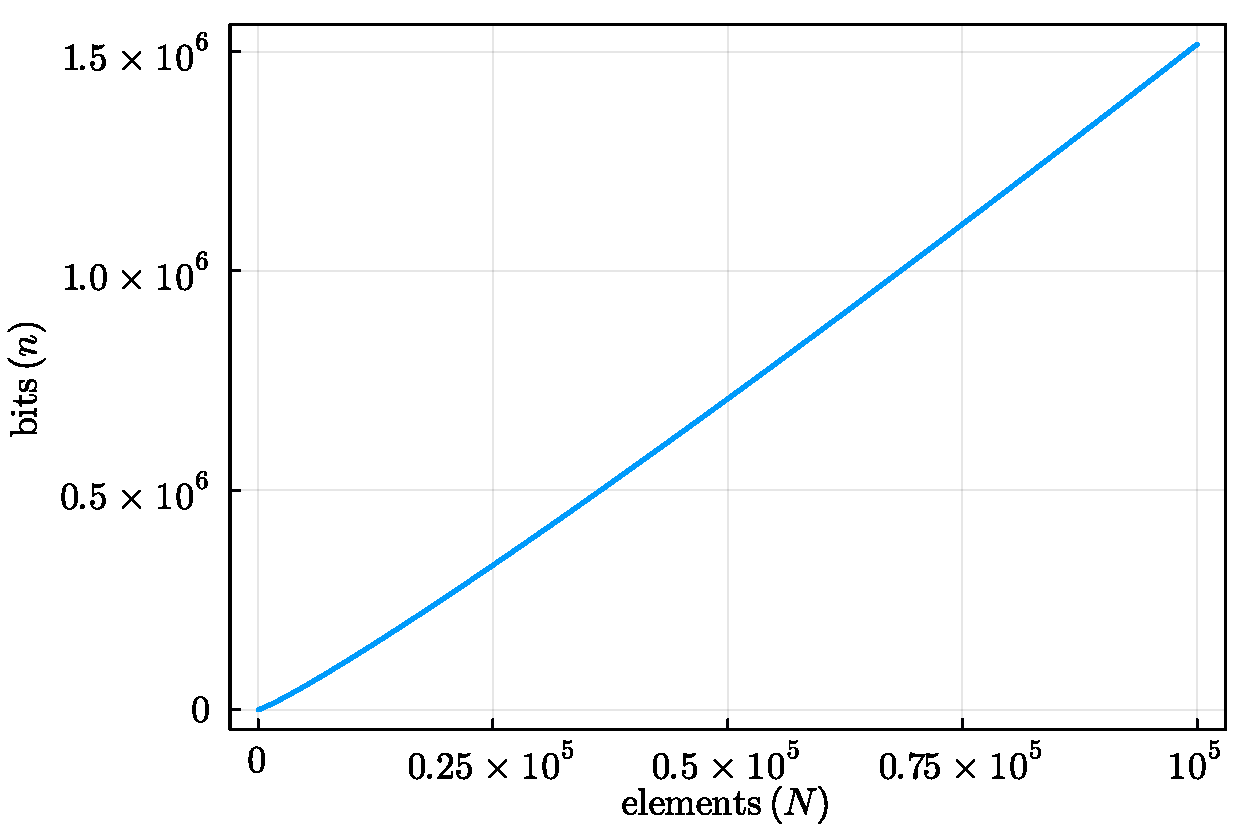
\includegraphics[width=\columnwidth]{figs/bits_permutations.pdf}
	\caption{\textbf{Number of bits ($n$) required to encode an arbitrary permutation ($S_N$) over $N$ elements.} This upper-bounds the required number of bits to uniquely address elements of the consensus group, $C(d)$.} \label{fig:bits_permutations}
\end{figure}